%Publication version
% \documentclass[aps,twocolumn,prd,superscriptaddress,showpacs,nofootinbib,fixfloat]{revtex4-1}
%Draft version
\documentclass[aps,prd,superscriptaddress,showpacs,nofootinbib,fixlfloat, 12pt]{revtex4-1}
%\usepackage{doublespace}
\usepackage{graphicx}
\usepackage{dcolumn}
\usepackage{bm}
\usepackage{natbib}

%\topmargin+1cm

\hyphenation{CTBCORE}

% Journals
\newcommand{\aaps}{{Astron.~Astrophys.~Supp.}}
\newcommand{\physrep}{{Physics~Reports}}
\newcommand{\araa}{{Annu.~Rev.~Astron.~Astrophys.}}
\newcommand{\aap}{{Astron.~Astrophys.}}
\newcommand{\apjl}{{Astrophys.~J.~Lett.}}
\newcommand{\apjs}{{Astrophys.~J.~Supp.}}
\newcommand{\aj}{{Astron.~J.}}
\newcommand{\mnras}{{Mon.~Not.~R.~Astron.~Soc.}}


% Making life easier
\newcommand{\be}{\begin{equation}}
\newcommand{\ee}{\end{equation}}
\newcommand{\bea}{\begin{eqnarray}}
\newcommand{\eea}{\end{eqnarray}}
\newcommand{\backten}{\!\!\!\!\!\!\!\!\!\!}


% useful symbols
\newcommand{\nhat}{\hat{\bf n}}
\newcommand{\kvec}{{\bf k}}
\newcommand{\edm}{\epsilon_{dm}}
\newcommand{\edmnow}{\epsilon_{dm,0}}
\newcommand{\sv}{\langle\sigma_Av\rangle}
\newcommand{\khat}{\hat{\bf k}}

% Fermi is usually italicized - use \Fermi\ for space after word
\newcommand{\Fermi}{{\slshape Fermi}}

% math functions, units
\newcommand{\Mpc}{{\rm ~Mpc}}
\newcommand{\sech}{{\rm ~sech~}}
\newcommand{\Tr}{{\rm ~Tr~}}
\newcommand{\threej}[6]{{\left( \begin{array}{ccc} #1 & #2 & #3 \\ #4 & 
   #5 & #6 \end{array} \right)}}

% Doug's units
\newcommand{\s}{{\rm ~s}}
\newcommand{\kms}{{\rm ~km/s}}
\newcommand{\g}{{\rm ~g}}
\newcommand{\cm}{{\rm ~cm}}
\newcommand{\ph}{{\rm ~ph}}
\newcommand{\sr}{{\rm ~sr}}
\newcommand{\km}{{\rm ~km}}
\newcommand{\mm}{{\rm ~mm}}
\newcommand{\mJy}{{\rm ~mJy}}
\newcommand{\Jy}{{\rm ~Jy}}
\newcommand{\MJy}{{\rm ~MJy}}
\newcommand{\MJypSr}{{\rm ~MJy~sr^{-1}}}
\newcommand{\JypSr}{{\rm ~Jy~sr^{-1}}}
\newcommand{\Hz}{{\rm ~Hz}}
\newcommand{\kHz}{{\rm ~kHz}}
\newcommand{\MHz}{{\rm ~MHz}}
\newcommand{\GHz}{{\rm ~GHz}}
\newcommand{\K}{{\rm ~K}}
\newcommand{\mK}{\rm ~mK}
\newcommand{\microK}{\mu{\rm K}}
\newcommand{\eV}{{\rm ~eV}}
\newcommand{\eVs}{{\rm ~eV/s}}
\newcommand{\keV}{{\rm ~keV}}
\newcommand{\MeV}{{\rm ~MeV}}
\newcommand{\GeV}{{\rm ~GeV}}
\newcommand{\TeV}{{\rm ~TeV}}
\newcommand{\pc}{{\rm ~pc}}
\newcommand{\kpc}{{\rm ~kpc}}
%\newcommand{\Mpc}{{\rm ~Mpc}}
\newcommand{\erg}{{\rm ~erg}}
\newcommand{\degree}{^{\rm o}}
\newcommand{\sigmav}{\langle\sigma_Av\rangle}
\newcommand{\zrock}{$Z_{\rm rock}$}
\newcommand\reftbl[1]{Table \ref{tbl:#1}}
\def\la{\vcenter{\hbox{$<$}\offinterlineskip\hbox{$\sim$}}}
\def\ga{\vcenter{\hbox{$>$}\offinterlineskip\hbox{$\sim$}}}
\newcommand\Refsec[1]{Section \ref{sec:#1}}

% Necessary for appendices

%% \newcommand\dpf[1]{{\bf (DPF: #1)}}
%% \newcommand\dpf[1]{{\bf (MS: #1)}}
%% \newcommand\dpf[1]{{\bf (CW: #1)}}

\begin{document}


\title{Let the LAT speak: Closing in on the Fermi line with a changed survey
strategy}

\author{Christoph Weniger}
\affiliation{GRAPPA Institute, Univ.~of Amsterdam, Science Park 904, 1098 GL
Amsterdam, Netherlands}

\author{Meng Su}
\affiliation{Institute for Theory and Computation,
  Harvard-Smithsonian Center for Astrophysics, 
  60 Garden Street, MS-51, Cambridge, MA 02138, USA} 
\affiliation{Department of Physics, and Kavli Institute for Astrophysics and Space Research, Massachusetts Institute of Technology, Cambridge, MA 02139, USA}
\affiliation{Einstein Fellow}

\author{Douglas P.~Finkbeiner}
%\email{dfinkbeiner@cfa.harvard.edu}
\affiliation{Institute for Theory and Computation,
  Harvard-Smithsonian Center for Astrophysics, 
  60 Garden Street, MS-51, Cambridge, MA 02138, USA} 
\affiliation{Center for the Fundamental Laws of Nature,
  Physics Department, 
  Harvard University, 
  Cambridge, MA 02138, USA}

\author{Torsten Bringmann}
\affiliation{II.~Institute for Theoretical Physics, University of Hamburg,
Luruper Chaussee 149, 22761 Hamburg, Germany}

\author{Nestor Mirabel}
\affiliation{affil}

%% Claims of a line are important and demand a careful search for
%% systematics.  Limb photons provide a reference spectrum and look a bit
%% fishy.  Need more data.
\begin{abstract} Coming soon...
\end{abstract}

\pacs{95.35.+d}

\maketitle


%%%%%%%%%%%%%%%%%%%%%% SECTION I %%%%%%%%%%%%%%%%%%%%%%%%%%%%%%%

\section{Introduction}
For indirect dark matter searches with gamma rays, discriminating between a
signal from conventional astrophysical backgrounds is challenging (for a
recent review see~\cite{Bringmann:2012ez}).  Among various possible
signatures, gamma-ray line emission is a long-sought ``smoking gun'' for dark
matter annihilation~\cite{Bergstrom:1988fp}, as no plausible astrophysical
background can produce a diffuse line signature.

% Gamma-ray line(s)
% could be produced by dark matter decays or annihilations
% into two photons, or two-body final states involving one
% photon plus a Higgs boson, Z boson, or other neutral non-SM
% particle.  In most models, the branching ratio
% to lines is loop suppressed relative to the continuum
% emission, and one would have expected to see the continuum
% first in e.g. MSSM models~\citep[e.g.][]{Bergstrom:1997}.
% Although this theoretical prejudice led most previous
% studies to focus on continuum searches, there are models
% being proposed that allow high line to continuum
% ratios~\citep[e.g.][]{Bergstrom:1998, Bergstrom:2000,
% Bertone:2009, Jackson:2010, Cline:2012, Weiner:2012}.
 
The first claims for a spectral feature around 130 GeV were made by Bringmann
\textit{et al.}~\citep{Bringmann:2012} and Weniger~\citep{Weniger:2012} (for
previous studies see~\cite{Pullen:2006sy, Abdo:2010nc, Vertongen:2011mu,
Ackermann:2012qk}). Subsequent work by Su \& Finkbeiner approached the problem
with template fitting, which takes into account the spatial distribution of
events along with spectral information, and found 6.6$\sigma$ (5.1$\sigma$
after the trials factor correction) for an Einasto profile centered
$1.5\degree$ west of the Galactic center, and also suggested that there may
be two lines, at about 111 and 129 GeV. The lower energy line is
tantalizing because it matches the expected energy of a $Z\gamma$ line if
the higher energy is the $\gamma\gamma$ line.  

% These findings have inspired a number of models and
% further analysis of the \Fermi\ data~\citep{Dudas:2012, Choi:2012,
% Kyae:2012, Lee:2012, Rajaraman:2012, Acharya:2012, Garny:2012,
% Buckley:2012, Chu:2012, Kang:2012, Buchmuller:2012, Bergstrom:2012b,
% Heo:2012, Park:2012, Tulin:2012, Cline:2012, Weiner:2012, WeinerYavin:2012b,
% FanReece:2012, Huang:2012, Whiteson:2012, Buchmuller:2012, Cholis:2012}.
 
% Recent evidence for lines at 111 GeV and 129 GeV with a
% local significance of $3.3\sigma$ from \Fermi\ unassociated
% point sources suggests an annihilation signal is
% present~\cite{doubleline}\citep[but
% see][]{HooperLinden:2012b}, as does the claim of line
% emission from galaxy clusters at 130
% GeV~\cite{Hektor:2012kc}.  Neither of these would stand on
% their own, but they provide support for the hypothesis that
% the Galactic center line signal is produced by dark matter
% annihilation.

% The high statistical significance of the line feature
% motivates a search for systematic errors in the LAT data
% that could mimic a line in the Galactic center.
% Confirmation by Imaging Air Cherenkov Telescopes like
% HESS-II might be possible as early as next
% year~\cite{Bergstrom:2012}, but in the meantime a thorough
% study of LAT systematics is urgently needed.  We do not have
% access to the details of the reconstruction of each photon
% event, which would allow us to study how it developed in the
% tracker and calorimeter.  However, we do have information
% about each event from the public event lists and spacecraft
% parameter files.  We can use this information to search for
% any line-producing artifacts in the detector frame, and
% investigate if they could map onto the Galactic center.
 
% The Earth's atmosphere provides a convenient source of
% photons for systematics tests.  The continual cosmic-ray
% cascades in the Earth's atmosphere produce gamma rays with
% $dN/dE \sim E^{-2.8}$~\citep{FermiLimb}.  Because these
% so-called `Earth limb photons' result from atmospheric
% cascades, they are produced by interactions in a highly
% boosted frame, and cannot contain line emission.
% \medskip

\dots Earth limb story etc \dots

\dots Here, we propose to settle this issue for good, using Fermi LAT itself
\dots

\section{Current status of signal and systematics}
Major concerns about the Galactic center signature are: (1) its statistical
robustness and (2) its possible cause by an instrumental systematic. We will
here shortly summarize the current situation, concentrating on statistical
properties of the Galactic center excess and -- as arguably the most worrisome
indication for a systematic -- the feature in the low incidence angle Earth
limb data.

\subsection{Time evolution of the signal significance}
The first claims of a spectral feature \citep{Bringmann:2012,Weniger:2012}
were based on 3.5 years of LAT data (through 4 February 2012).  Subsequent
data provide an opportunity to confirm the signal and see how it evolves with
time.  Because the signal is based on approximately 1 signal count per month
in the region of interested (ROI) that gave the highest significance, Poisson fluctuations cause the significance to accumulate in
something akin to a random walk.  The mean trend in significance builds with
sqrt(time) but with large uncertainties.  A confirmation at $3\sigma$ of the
signal in the original ROI (i.e.~no trials factor) would be persuasive, but
the exposure required to get an expected significance of $3\sigma$ is quite
different from the exposure required to achieve $3\sigma$ \emph{with 95\%
  probability.}

\begin{figure}[h]
  \begin{center}
    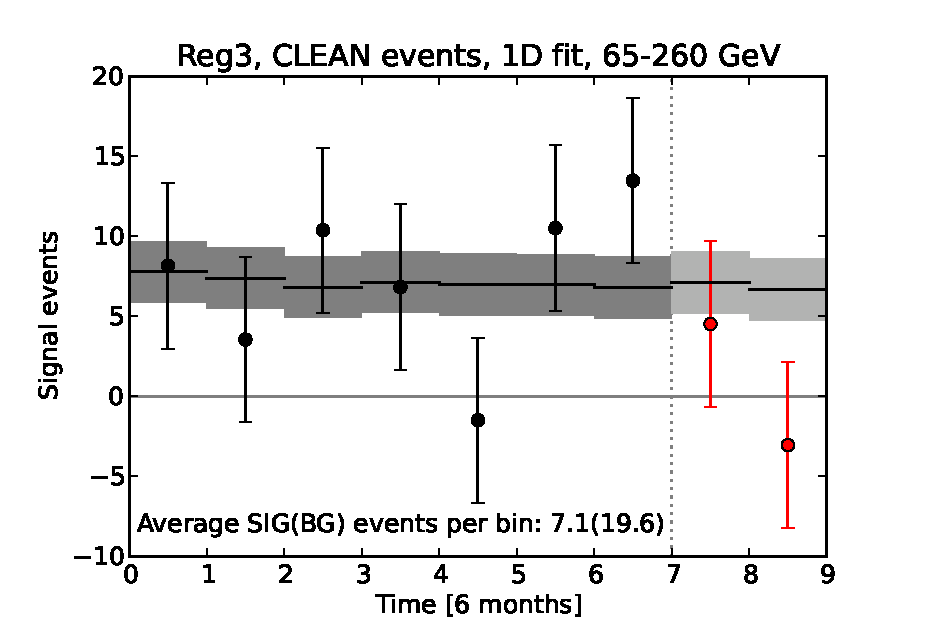
\includegraphics[width=0.60\linewidth]{plots/semester_fluxes.eps}
    \vspace{-0.5cm}
  \end{center}
  \caption{Number of signal events in 6-month bins starting from 4
    August 2008, obtained by an unbinned likelihood fit to the data in
    Region~3 of Ref.~\cite{Weniger:2012}. The gray band shows the expected
    signal rate with $\pm1\sigma$ uncertainty as extracted from data taken until
    4 February 2012; the small variations stem from variations of the
    exposure. In red we show data taken since 4 February 2012
    together with the projected event rate.}
  \label{fig:semester_fluxes}
\end{figure}

\begin{figure}[h]
  \begin{center}
    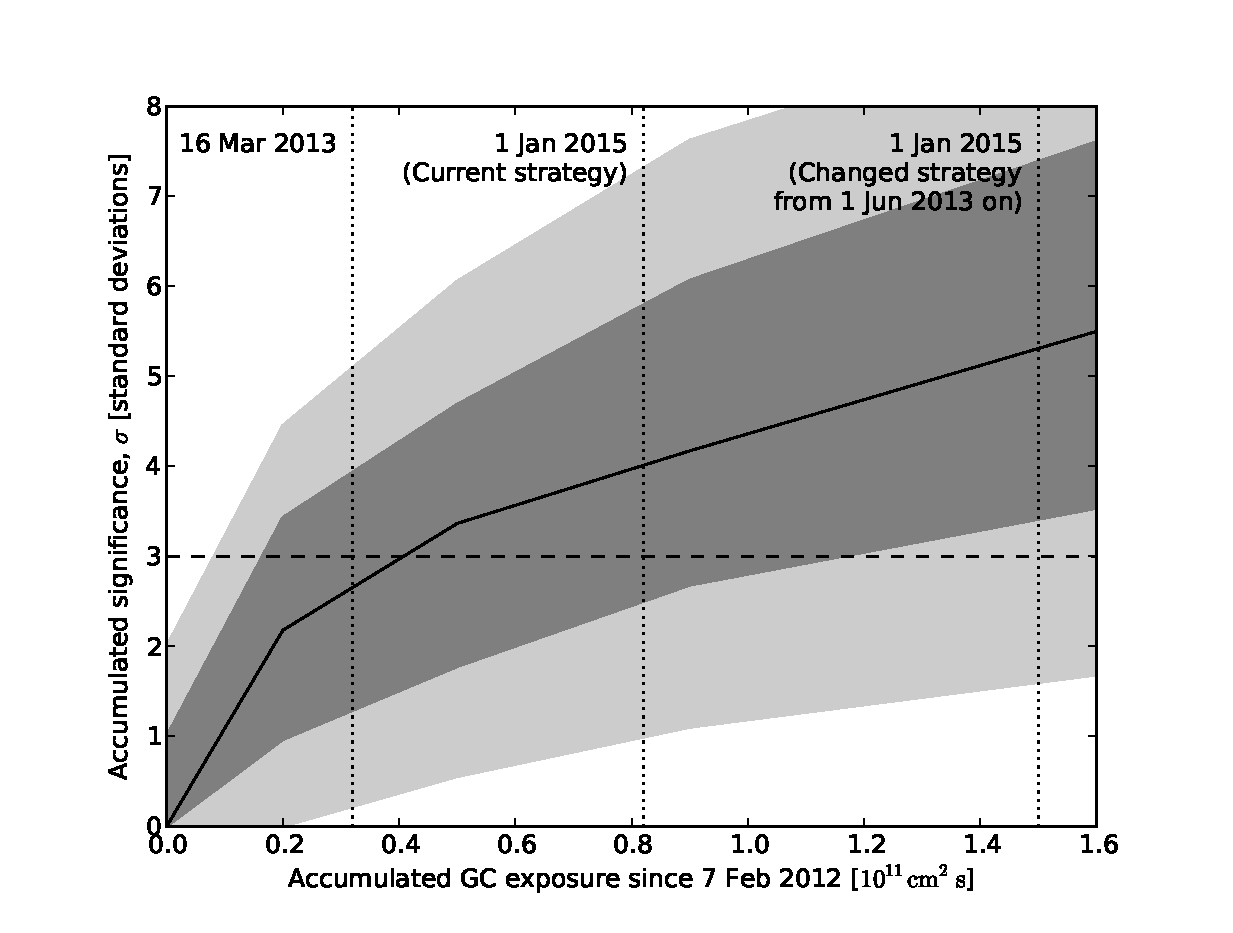
\includegraphics[width=0.6\linewidth]{plots/projection.eps}
    \vspace{-0.5cm}
  \end{center}
  \caption{
    \textbf{(Update figure with correct exposure factor for optionX)}
    Expected evolution of signal significance in Region~3 from
    Ref.~\cite{Weniger:2012}, starting on 4
    February 2012, as function of
    accumulated exposure.  The shaded bands show $68\%$ and $95\%$ CL
    uncertainties as derived from a Monte Carlo simulation.  The assumed
    signal rate is $1.2\pm 0.3$ events per month, the effective background is
    $3.3$ events per month (the values measured prior to 4 February 2012).
    The first and second vertical dotted lines indicate how much exposure is
    expected to be accumulated until end of 2014 if the observation strategy remains
    unchanged, and respectively when the observation strategy proposed in this
    document is adopted starting from June 2013.}
  \label{fig:projection}
\end{figure}

\begin{figure}[h]
  \begin{center}
    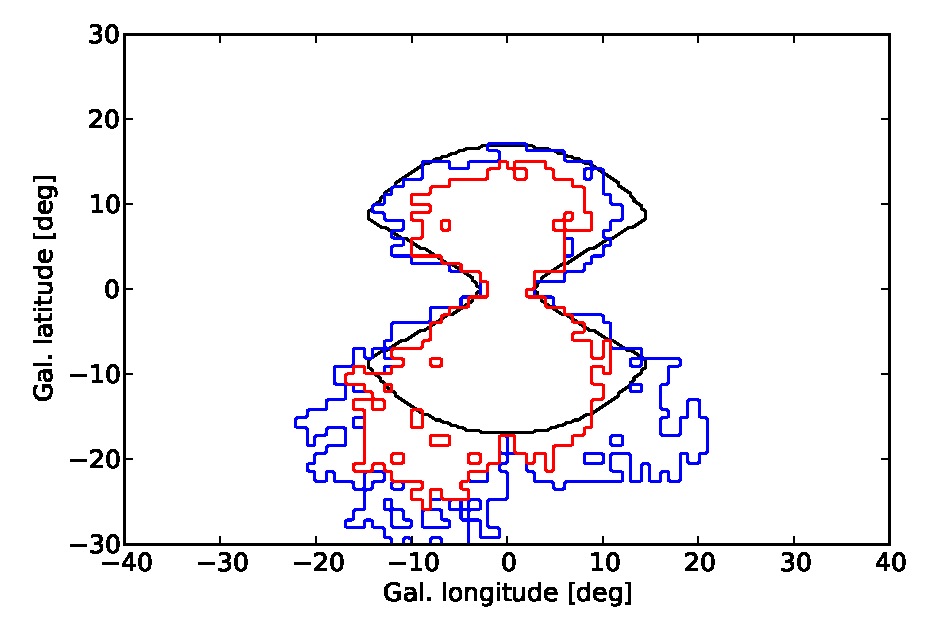
\includegraphics[width=0.6\linewidth]{plots/regions.eps}
    \vspace{-0.5cm}
  \end{center}
  \caption{Region 3 (blue) and Region 4 (red) used in
    Ref.~\cite{Weniger:2012}, together with the simpler hourglass region
    proposed for future studies.}
  \label{fig:projection}
\end{figure}

\emph{Status.} In order to discuss the statistical robustness of the GC
signature, we use the first 3.5 years of data, taken since 4 August 2008, to
define the spectral and spatial properties of our signal hypothesis (this is
the data set that was used in the initial publication,
Ref.~\cite{Bringmann:2012}). Data taken after the 4 February 2012 can then be
used to confirm or reject this hypothesis without trials. To be conservative,
we will not use the template regression technique from Ref.~\cite{linepaper},
but follow~\cite{Bringmann:2012, Weniger:2012} and use spectral fits in ROIs
with large S/N.  For definiteness, we will here only use `Region 3' from
Ref.~\cite{Weniger:2012}; this is one of the regions where the excess was
first identified with high significance. Below we will
propose a geometrically similar but much simpler region that we advocate as an
alternative for future studies.
% The temporal distribution of `signal' events at the Galactic center over the
% previous 4.5 years of data taking can be used for a trial-free statistical
% confirmation of the excess. 

% The number of signal events $N_s$ in each bin follows directly from a
% maximum likelihood fit to the data (power-law background plus line feature). 
We derive the number of excess events $N_s$ by a maximum likelihood fit to the
first 3.5 years of data from Region 3 (using a power-law plus line model). In
the fit, we adopt an energy range from 65 to 260 GeV, fix the line position at
$E_\gamma=129.8\rm\,GeV$, and use P7CLEAN events only.\footnote{The details of
the fit are identical what was done in Ref.~\cite{Weniger:2012}, but we
checked that similar results are obtained using Region 4, P7SOURCE events,
or a `2D' fit that takes into account incidence angle as well as energy
information in the modeling of the line.} We find a number of $N_s=50.0\pm 13.3$
excess events (with $\pm1\sigma$ profile likelihood errors), with a
statistical significance of $s=4.3\sigma$. The effective number
of background events can estimated as $N_b = N_s^2/s^2$, and is $N_b=137.4$.
These parameters together with the details of the fit define our \emph{signal
hypothesis}; the \emph{null hypothesis} is that the flux is compatible with a
single power law, i.e.~$N_s=0$.

In Fig.~1 we show the distribution of these excess events in bins of six
month. The first seven bins correspond to the 3.5 years that define the
excess, the two red data points are data taken afterwards. Error bars include
background fluctuations and are given by $\Delta N_s = \sqrt{N_s+N_b}$. To
obtain $N_s$ and $N_b$, we fit the data from each six month interval
individually. The gray bands show the number of signal events expected from
the above fit to the 3.5 years data, with small variations being related to
the exposure.

The last two bins are compatible with both the null-hypothesis at the one
sigma level, and with the signal-hypothesis at the two sigma level (see also
Ref.~\cite{Weniger:2013dya}). In case of a real signal, the last bin would
represent a decent downward fluctuation. However, it is premature to
draw strong conclusions from this single downward fluctuation.

\emph{Projection.} 
Going forward, the signal hypothesis predicts that the significance will build
as sqrt(exposure), but with large uncertainties.  It is essential to estimate
these uncertainties, because we need to know how much exposure is required to
\emph{cleanly} separate the signal hypothesis from the null hypothesis. 

In Fig.~2 we show 68\% and 95\% CL bands for the projected evolution of the
signal significance as function of exposure accumulated after 4 February 2012.
To generate the plot, we simulate events from a power-law plus line model and
derive the signal significance for each realization as described above. The
background and signal correspond to the best-fit values obtained in Region 3
with data until 4 February 2012.  For different realizations we allow the
signal normalization to vary following a normal distribution that is matched
to the $\pm1\sigma$ flux uncertainties from the 3.5 year results.\footnote{We
checked that similar results for the projection evolution are obtained for
Region 4, or in the hourglass region discussed below.}

The first vertical dashed line indicates the exposure that will be acquired by
1 Jan 2015 with the current survey strategy. It is likely that a true signal
would be confirmed with $>3\sigma$ significance, although this is not
guaranteed due to the $95\%$ CL error bands that range down to significances
of only $1\sigma$. Worse, it will be difficult to robustly rule out the signal
hypothesis at the $3\sigma$ level unless the accumulated significance is close
to zero.  This drives home the point that, left unchanged, the current survey
strategy may well leave us with ambiguous results well into 2015.  As we will
discuss in the next section, a change in the observation strategy will allow a
much quicker confirmation/rejection of the signal hypothesis.
\medskip

\emph{Alternative ROI.} For future analysis of the 130 GeV feature in the LAT
data, instead of using the difficult to manage regions from
Ref.~\cite{Weniger:2012}, we propose to use the region shown in black in
Fig.~3. This region is (1) geometrically simple and easy to reproduce, and (2)
it is centered on the part of the sky where the excess was largest in the
previous data. Though we avoid any statement about particular dark matter
profiles, it is an \emph{a priori} region for data taken since 4 February
2012. We defined this ROI in $(\ell, b)$ space as the intersection of
$\ell^2+b^2\leq
r^2$ and $\ell^2\leq (b\tan\varphi)^2 + d^2$, with $(r, d, \varphi) =
(20^\circ, 3^\circ, 60^\circ)$. 
%and note that it has similar signal-to-noise
%properties as Region 3 or 4. 

\subsection{The Earth limb feature}
The most direct indication for an instrumental cause of the Galactic center
feature is an excess of 130 GeV photons in low incidence angle events from
the Earth limb~\cite{linepaper, finkbeiner_systematics, Hektor:2012ev,
bloom_charles_fermi_lat_line}. Although it is challenging to understand how
such a feature could possibly be mapped onto the Galactic center while being
absent in other test regions, this feature raised serious concerns about the
energy reconstruction of the LAT around 130 GeV.  Additional limb data would
determine whether the Earth limb feature is indeed a true systematic effect or
merely a statistical fluke in light of a large number of hidden trials.

We define here the Earth limb excess by selecting P7CLEAN events until 5 Sep 2012 at zenith angles $Z>100^\circ$,
incidence angles $\theta<60^\circ$, and excluding events within $20^\circ$ of
the Galactic center. In this data set, the line feature at 130~GeV has a
significance of $2.7\sigma$ when
adopting an energy range from 65--260~GeV in the fit (for details of the
assumed line shape, etc.,
see Ref.~\cite{finkbeiner_systematics}).\footnote{If we take into account data
  until 16 Apr 2013, the
significance of the Earth limb feature is $3.0\sigma$, which is marginally
larger.}
Data accumulated after 5 Sep 2012 can
now be used to test whether this excess is a fluke or not. Using the above
cuts, we find that the rate of events above 100 GeV that were accumulated between the
start of the mission and 5 Sep 2012 is 9.5 ph/month (in total 474), whereas it
was 36.7 ph/month between 5 Sep 2012 and 16 Apr 2013. The reason for this increase
in the rate are the start of weekly dedicated limb observations as well as two extended
target of opportunity observations in that time period. If the accumulation of
low incidence angle Earth limb data continues at this pace, 2.3 years of fresh
data are enough to regenerate the putative signature with $4.0\sigma$
significance \emph{on average}, or to rule it out with high significance if it is a
fluke. Without a change of the observation strategy, this amount of data would
be available end of 2014. As we will discuss next, a change of the
observation strategy would help to collect the same amount of low incidence
angle Earth limb data in a much shorter time period.



\begin{figure}[t]
  \begin{center}
    \includegraphics[width=0.49\linewidth]{plots/survey_lineEval.eps}
    \includegraphics[width=0.49\linewidth]{plots/option3v3_lineEval.eps}
    \vspace{-0.5cm}
  \end{center}
  \caption{Evaluation of standard survey mode (\emph{left panels}) and mixed observation
    strategy (\emph{right panels}). Sky maps are in galactic coordinates ($\ell$ increases
    to the left) and averaged over a orbital precession period of 55 days.
    \emph{Top
      panels:} Exposure maps in cm$^2$s.
    \emph{Central panels:}
    Effective energy resolution (half 68\% containment width)
  \emph{Bottom panels:} Figure of merit for gamma-ray line searches. In all
  panels the overlaid lines show the main axes of the equatorial coordinate
  system; sky maps are symmetric around the celestial equator.}
  \label{fig:mollweide}
\end{figure}

\begin{figure}[t]
  \begin{center}
    \includegraphics[width=0.49\linewidth]{plots/option1v2_lineEval.eps}
    \includegraphics[width=0.49\linewidth]{plots/option2v2_lineEval.eps}
    \vspace{-0.5cm}
  \end{center}
  \caption{Same as Fig.~\ref{fig:mollweide}, but for 'option1v2' and
  option2v2'.}
  \label{fig:mollweide2}
\end{figure}

\section{A New Observation Strategy}
Since the start of the mission, Fermi has spent over 95\% of the time in
\emph{standard survey mode}.
% With a field of view of $\sim2.5$~sr, the LAT can survey the entire sky in
% two orbits. 
In this mode, the LAT points north of zenith towards the orbital pole by an
angle \zrock\ on one orbit, and south of zenith by the same angle on the next
orbit; the LAT pointing is confined to the plane perpendicular to its orbital
velocity. 
This observation profile, combined with the precession of the orbit every
$\sim53.4$ days, allows the LAT to observe the whole sky with approximately
uniform coverage. The standard survey mode is only occasionally interrupted
for pointed observations of targets of opportunity (ToOs). During such times
the LAT may point at a larger zenith angle than usual, even at the horizon.  In
addition, survey mode is occasionally interrupted by Autonomous Repoints of
the observatory for triggered gamma-ray burst follow-up observations, and for
calibration.
% Furthermore, \Fermi's survey observations are halted during passages through
% the South Atlantic Anomaly, resulting in an exposure differential between
% north and south of $\sim15$\%. 

However, Fermi is capable of very flexible survey mode patterns. For example,
a single orbit may include both survey mode and pointed observations (``mixed
mode''), increasing coverage of certain parts of the sky. We will explore the
impact of such a strategy on study of the 130 GeV feature at the Galactic
center.  We focus here on the mixed modes ``option1v2'', ``option2v2'' and
``option3v3'' put forth for discussion by the Fermi mission.\footnote{See
\url{http://fermi.gsfc.nasa.gov/ssc/proposals/alt_obs/obs_modes.html}.}

We are interested in increasing the exposure of the Galactic center.  The
basic strategy would be to switch to pointed observation of the Galactic
center when possible, and to follow the standard survey mode otherwise. More
precisely, \Fermi\ would slew from survey mode to the target once the target
is $10^\circ$ from Earth occultation, and slew back to survey mode position
once the target reenters $10^\circ$ from Earth occultation.  The minimal
distance to the Earth horizon (the Earth Avoidance Angle, EAA) is set to
$30^\circ$, to avoid the loss of too much exposure during the transition
periods. 

To reduce potential systematics, it is advisable to avoid pointing directly at
the target. Instead, it is useful to observe it with a broad distribution of
non-zero incidence angles. The three mixed modes ``option1v2'', ``option2v2''
and ``option3v3'' differ mainly in what target position exactly is adopted.
In ``option1v2'' and ``option2v2'', the target position is fixed at (RA,
Dec)=($261.4^\circ$, $-28.9^\circ$) and (RA, Dec)=($261.4^\circ$, $0^\circ$),
respectively.  In ``option3v3'' the target position RA is set to
261.4$^\circ$, while the target position declination oscillates within the
range Dec=$\pm25.6^\circ$ during one orbital precession period such that the
target position lies on the orbital equator.  The variation of the target
position yields an improved sky uniformity on short time scales. 

\subsection{Impact on line searches at the GC}
The upper panels of Fig.~\ref{fig:mollweide} show exposure maps after 55 days
survey mode (left) and mixed mode ``option3v3'' (right) in galactic
coordinates.  In the mixed mode, the point of highest exposure is at (RA,
Dec)$\simeq(261.4^\circ$, $0^\circ)$. At the GC, the exposure increases by a
factor of 2.23 with respect to normal survey mode.

In mixed mode, regions close to the GC are predominantly observed
under low incidence angles in the range $\theta=4^\circ$--$54^\circ$ (see
Fig.~\ref{fig:thetaDist}). This has impact on the effective energy resolution,
which is shown in the central panel of Fig.~\ref{fig:mollweide}. In direction
of the GC the energy resolution is in fact slightly worsen with respect to the
standard survey mode ($\Delta E/E=9.59\%$ instead of $\Delta E/E=8.75\%$).
However, this loss of resolution has only a small effect on line searches.

In Fig.~\ref{fig:mollweide2}, we show the same information, but for the mixed
modes option1v2 (left) and option2v2 (right). The GC exposure increases by a
factor XXX and XXX, respectively, whereas the effective energy resolution is
$XXX$ and $XXX$. Apart from the characteristics at the GC, these modes mainly
differ in the impact on other science goals, as we will discuss below.
\medskip

As a convenient \emph{figure of merit} for line searches we define the
dimensionless quantity $$Q\equiv a\sqrt{\mathcal{E}/\Delta E}\,,$$ which is
proportional to the expected median line significance in units of standard
deviations.  Here, $\mathcal{E}$ is the exposure in cm$^2$s, and $a$
normalizes $Q$ such that the spatial mean in survey mode is $\bar Q=1$. In the
bottom panel of Fig.~\ref{fig:mollweide} we show sky maps for $Q$ in mixed and
survey mode.  At the Galactic center, $Q$ increases by a factor $1.43$ when
switching to mixed mode observation, which would increase the growth rate of
the signal significance by $43\%$, equivalent to doubling the exposure/time. 

\subsection{Impact on Earth limb observations}
An important side effect of the mixed mode is the accumulation of
additional Earth limb data at low incidence angles, which can be used for
checks of instrumental systematics. This happens during the
transitions between pointed observation and survey mode. The target comes
close to the horizon, while the satellite maintains a minimal distance of
$30^\circ$ from the Earth limb. Consequently, the Earth limb is observed at
incidence angles $\theta\gtrsim30^\circ$ twice every orbit (1.5 hours).

In Fig.~\ref{fig:limb_exposure}, we show the expected differential exposure of
the Earth limb at zenith angles $111^\circ<Z<113^\circ$. In standard survey
mode, practically no limb data is collected at $\theta\lesssim60^\circ$.
However, during mixed mode a very significant number of the detected Earth
limb events would be collected at lower incidence angles. This would
accelerate the accumulation of low incidence angle Earth limb data with
respect to the previous 4.5 years by about \emph{a factor of five}, and will
allow a rapid rejection or confirmation of the 130 GeV feature in part of the
Earth limb spectrum. Note that a collection of Earth limb events at incidence
angles even lower than $30^\circ$ is possible if the EAA is set appropriately,
however at the cost of losing more exposure on the rest of the sky.

\begin{figure}[t]
  \begin{center}
    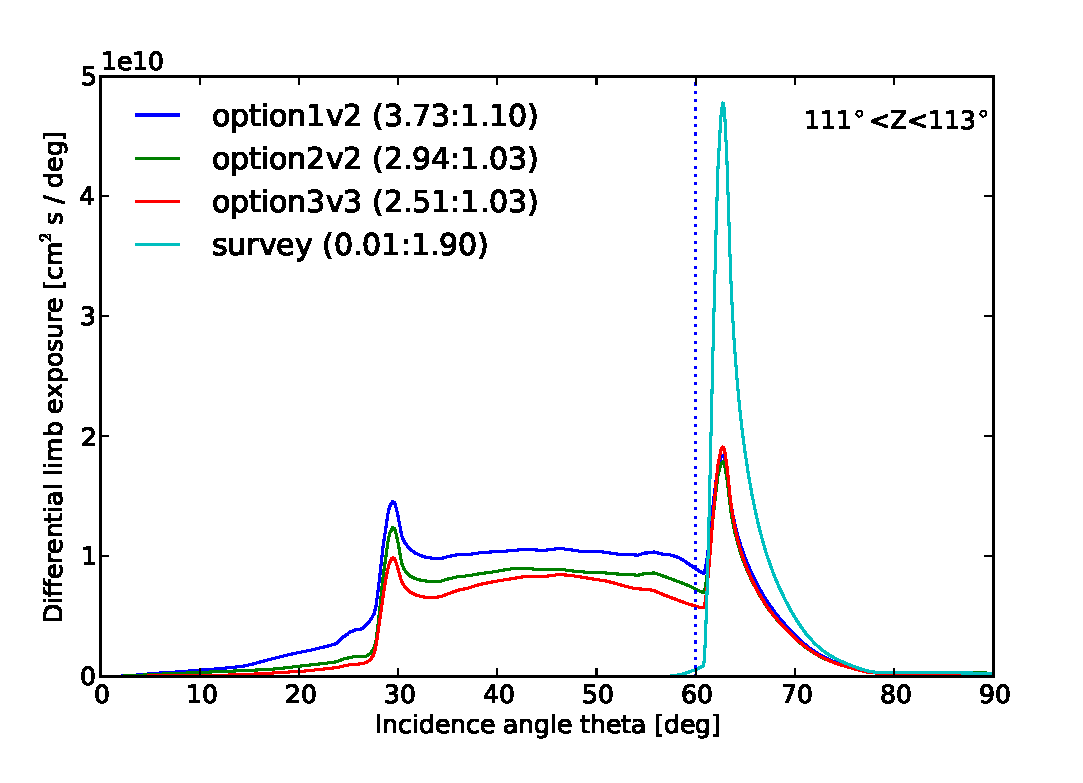
\includegraphics[width=0.6\linewidth]{plots/limb_exposure.eps}
    \vspace{-0.5cm}
  \end{center}
  \caption{Differential exposure of Earth limb region (zenith angles
    $111^\circ<Z<113^\circ$) as function of incidence angle $\theta$. In
    standard survey mode, incidence angles below $\theta<60^\circ$ are not
    exposed to the Earth limb. However, in mixed observation modes, a
    large number of Earth limb events would be collected down to incidence
    angles $\theta\simeq30^\circ$. In brackets we show the exposure below and
  above $\theta=60^\circ$ in units of $10^{11}\rm\,cm^2\,s$.}
  \label{fig:limb_exposure}
\end{figure}


\subsection{Impact on other science}

\begin{figure}[t]
  \begin{center}
    \includegraphics[width=0.39\linewidth, angle=-90]{plots/option1_survey_hist.ps}
    \includegraphics[width=0.39\linewidth, angle=-90]{plots/option2_option3_hist.ps}
    \vspace{-0.5cm}
  \end{center}
  \caption{Histogram of exposure per sky pixel, normalized to standard survey
    strategy \textbf{(it does not look like that!)}. Left panel compares the
    mixed mode option1v2 to the standard survey strategy, and the right panel
    shows the modified strategy option2v2 and option2v3.}
  \label{fig:expHisto}
\end{figure}
Changing from survey mode to mixed mode observation will necessarily drag
exposure from some parts of the sky towards the Galactic center. In order not
lower the scientific power of Fermi, the \emph{integrated} exposure over the
whole sky should however remain as high as possible.  Furthermore, for the
observation of transient phenomena, it is vital that all parts of the sky are
sufficiently covered at least each day; `blind spots' should be avoided.

\begin{table}[t]
  \begin{tabular}{lcrcr}
    Mode && Integrated exposure && GC exposure \\
    survey && 5.54e9 && \\
    option1v2 && 5.13e9 && \\
    option2v2 && && \\
    option3v3 && && \\
%     % survey
  \end{tabular}
  \caption{This is the caption}
\end{table}

In Fig.~\ref{fig:expHisto}, we show a histogram of the distribution of
exposure in different pixels of the sky (using a Healpix projection with
$N=128$). In the case of standard survey mode, the exposure distribution spans
a factor of two, whereas it spans a factor $12$ in the mixed observation mode. 
% However, only in a small fraction of the sky, about XXX\%, the coverage
% drops by as much as a factor of $0.3$--$0.5$, and never below $0.3$.


In Fig.~\ref{fig:coverage} we
show for each individual day of the precession period which fraction of the
sky is covered by what fraction of the mean exposure. As can be seen from the
plot, in less than $\sim5\%$ of the sky the daily coverage drops below $20\%$
of the mean, whereas in $>80\%$ the daily coverage remains above $50\%$ of the
mean.

\dots comparison of exposure integrated over whole sky for different options \dots

\subsection{Possible triggers}
{\bf moved here from the end, where it did not belong.  Remove entirely??}
A more conservative approach might involve waiting for certain triggers before
initiating a change.  For example, one might wait until the Pass 8 processing
is finished before making the change.  However, it will probably not be public
for another year or more, and we feel it is undesirable to tie this decision
to a data release at an uncertain date.  It is also difficult to tie the
decision to an internal release; in order for the community to provide input,
the decision must be made based upon public data. 

Another trigger might be to just wait until X significance is achieved.  This
could cause a long-enough delay to make a later change insufficient.  And this
is seems backwards.  It would make more sense to make the change immediately,
and then have a trigger to revert to normal survey mode when the signal
hypothesis is ruled out at some level.


\begin{figure}[t]
  \begin{center}
    \includegraphics[width=0.38\linewidth, angle=-90]{plots/exposure_pixel_hist_perday_option1.ps}
    \includegraphics[width=0.38\linewidth, angle=-90]{plots/exposure_pixel_hist_perday_option2.ps}
    \includegraphics[width=0.38\linewidth, angle=-90]{plots/exposure_pixel_hist_perday.ps}
    \includegraphics[width=0.38\linewidth, angle=-90]{plots/exposure_pixel_hist_perday_survey.ps}
    \vspace{-0.5cm}
  \end{center}
  \caption{Daily sky coverage with different range of exposure
  time normalized to the mean value of the exposure map of each day (in total
  55 days to complete on orbit precession period).} 
  \label{fig:coverage}
\end{figure}

\dots theta distribution at GC (optional) \dots

\begin{figure}[t]
  \begin{center}
    \includegraphics[width=0.38\linewidth, angle=-90]{plots/option1v2_theta.ps}
    \includegraphics[width=0.38\linewidth, angle=-90]{plots/option2v2_theta.ps}
    \includegraphics[width=0.38\linewidth, angle=-90]{plots/option3v3_theta.ps}
    \includegraphics[width=0.38\linewidth, angle=-90]{plots/survey_theta.ps}
    \vspace{-0.5cm}
  \end{center}
  \caption{The distribution of Galactic center theta angle. Each entry in the
  histogram corresponds to a 30 seconds interval. The two colors correspond to
  different ranges from the GC and to the Fermi zenith angle.
  Note that this includes time in the SAA.} %Right panel: in stead the sky
  %coverage, we plot the fractional exposure time relative to the mean value of
  %the exposure map of each day.}
  \label{fig:thetaDist}
\end{figure}

\begin{figure}[t]
  \begin{center}
    \includegraphics[width=0.9\linewidth, angle=0]{plots/transient_source_map.ps}
    \vspace{-0.5cm}
  \end{center}
  \caption{The spatial distribution of 1FAV sources overplotted with the exposure map of Option 1 survey strategy. Red circles mark sources with expected exposure $>150\%$ than the standard survey strategy with a total number of 25 sources. Green circles mark sources with expected exposure $<50\%$ than the standard survey strategy with a total number of 59 sources. The rest sources are marked by blue cycles in total 131. }
  \label{fig:transmap}
\end{figure}

\begin{figure}[t]
  \begin{center}
    \includegraphics[width=0.7\linewidth, angle=-90]{plots/source_type_hist.ps}
    \vspace{-0.5cm}
  \end{center}
  \caption{Source type distribution for the 1FAV catalog. We classify the sources into three categories: sources with expected exposure time (assuming option 1 survey strategy) less than 50\% of the standard survey strategy; sources with expected exposure between 50\% to 150\% compared to the standard survey strategy; and sources with expected exposure more than 150\%. }
  \label{fig:transhist}
\end{figure}


\section{Discussion and Conclusion}
\label{sec:Conclusion}

In this document we have argued for a change in the Fermi survey strategy to
increase exposure in the inner Galaxy, and confirm or rule out claims of a 130
GeV spectral line.  The principal reasons for a change are:

\begin{itemize}

\item{\bf It is important: discovery of a dark matter annihilation line in the
    Galactic center would be Fermi's greatest accomplishment.}  The nature of
  dark matter is one of the greatest mysteries in physics and astrophysics,
  and the discovery of a line would be a major step forward for both fields.
  Exploring the nature of dark matter is one of the major goals of the Fermi
  project, and a discovery would define Fermi's legacy.

\item{\bf Fermi can do it: a modified survey strategy can obtain a decisive
    measurement, while the status quo may not.}  The significance of a line
  evolves as sqrt(exposure), but with large uncertainty due to Poisson
  fluctuations.  For example, if the signal hypothesis is correct, the
  expected signal significance by 1 Jan 2015 is about $4\sigma$
  (Fig. \ref{fig:projection}).  Poisson fluctuations broaden this range such
  that the actual significance achieved is between 2.5 and
  5$\sigma$ 68\% of the time, and between 1.5 and 6.5$\sigma$ 95\% of the
  time.  A clear separation of the signal hypothesis from the null hypothesis
  requires more data than one might think.  If the project continues with
  standard survey mode until 2016, there is a fair chance that we leave this
  question unresolved.  We cannot permit this to happen.

\item{\bf This is a win-win: the proposed change is not bad for other science.}  There will be winners and
  losers in any change, but more time on the inner Galaxy is good for lots of
  projects (better time coverage for pulsars and transients, etc.).  Many
  wide-angle surveys (SDSS, Pan-STARRs, etc.) have found it fruitful to
  dedicate a significant fraction of observing time to ``deep fields'' where
  greater sensitivity and improved cadence extend the range of phenomena
  observable.  Furthermore, roughly half
  the sky has more exposure under the new strategy, and even the underexposed
  regions are still observed on a regular basis for continued monitoring of
  transients (Fig. \ref{fig:coverage}).

\end{itemize}

For all of these reasons, we advocate a change in the survey strategy, as soon
as possible.
{\bf (Should we specifically advocate option 3 here?)  }


At least for the next several years, Fermi is uniquely able to address the 130
GeV line.  If it is an artifact, it is a subtle one -- and understanding its
origin is important for the dark matter search in
particular, and the mission as a whole.  If the line is real, we would forever
regret missing this opportunity to pursue it aggressively. 

\clearpage
\bibliography{whitepaper}

\end{document}
